\documentclass[14pt]{extarticle}
\usepackage[T1]{fontenc}
\usepackage[default]{sourcesanspro}
\usepackage[letterpaper,top=0.75in,bottom=0.75in,left=0.65in,right=0.65in,
  headheight=18pt,headsep=0.28in,footskip=0.45in]{geometry}
\usepackage{tikz}
\usepackage{fancyhdr}
\usepackage[none]{hyphenat}
\usepackage{ragged2e}
\definecolor{cube}{RGB}{176,204,236}
\definecolor{folder}{RGB}{240,218,166}
\pagestyle{fancy}
\fancyhf{}
\fancyhead[L]{Week 5 / Tower cities / Grades 2--3}
\fancyfoot[L]{Bellingham Math Circle / Week 5 / F05-M-v4}
\fancyfoot[R]{\thepage}
\renewcommand{\headrulewidth}{0.4pt}
\renewcommand{\footrulewidth}{0pt}
\setlength{\parindent}{0pt}
\setlength{\parskip}{0pt}
\raggedbottom
\RaggedRight
\newcommand{\prob}[1]{\textbf{Problem #1:}\ }
\begin{document}
Look along a row of towers from one end, with your eye down at the table about a foot away. You see a tower when it is taller than every tower in front of it.
\par\vspace{0.6cm}
\begin{minipage}{\linewidth}\RaggedRight
\prob{1}Stand towers of 1, 2, and 3 cubes in a row. Find every order of the three towers, and write each one with the number of towers seen from each end. Which pairs of numbers can a row of three towers never show? Explain why.
\vspace*{0.2cm}
\begin{center}
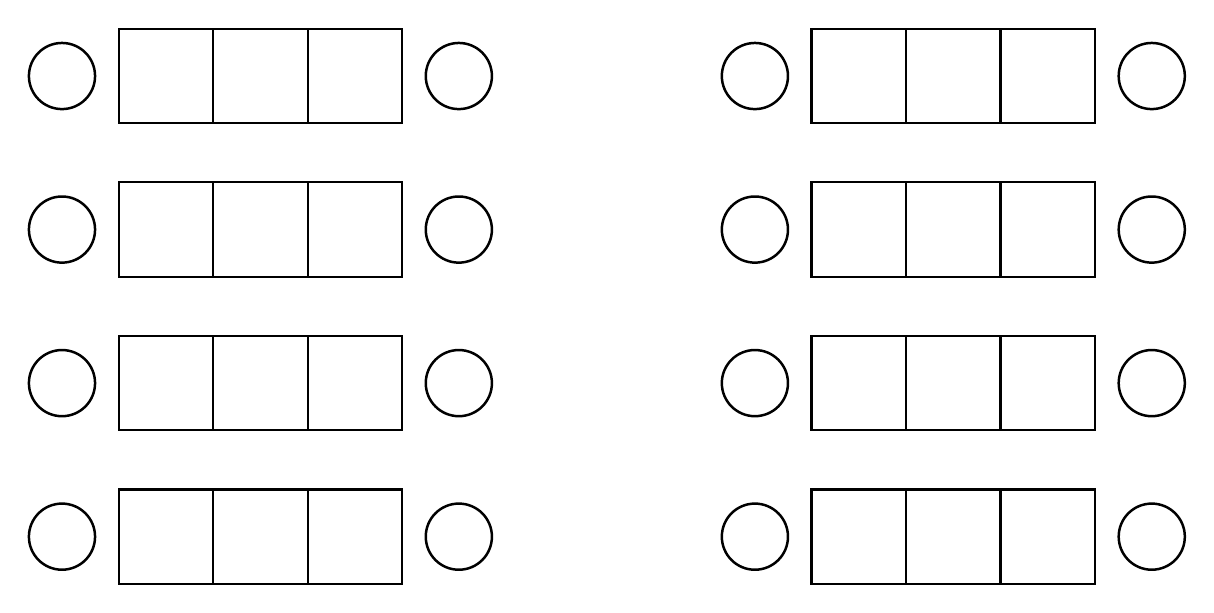
\begin{tikzpicture}
\begin{scope}[shift={(0.000,0.000)}]
\draw[line width=0.8pt] (0.000,0) rectangle (1.200,1.200);
\draw[line width=0.8pt] (1.200,0) rectangle (2.400,1.200);
\draw[line width=0.8pt] (2.400,0) rectangle (3.600,1.200);
\draw[line width=0.9pt] (-0.720,0.600) circle (0.420);
\draw[line width=0.9pt] (4.320,0.600) circle (0.420);
\end{scope}
\begin{scope}[shift={(8.800,0.000)}]
\draw[line width=0.8pt] (0.000,0) rectangle (1.200,1.200);
\draw[line width=0.8pt] (1.200,0) rectangle (2.400,1.200);
\draw[line width=0.8pt] (2.400,0) rectangle (3.600,1.200);
\draw[line width=0.9pt] (-0.720,0.600) circle (0.420);
\draw[line width=0.9pt] (4.320,0.600) circle (0.420);
\end{scope}
\begin{scope}[shift={(0.000,-1.950)}]
\draw[line width=0.8pt] (0.000,0) rectangle (1.200,1.200);
\draw[line width=0.8pt] (1.200,0) rectangle (2.400,1.200);
\draw[line width=0.8pt] (2.400,0) rectangle (3.600,1.200);
\draw[line width=0.9pt] (-0.720,0.600) circle (0.420);
\draw[line width=0.9pt] (4.320,0.600) circle (0.420);
\end{scope}
\begin{scope}[shift={(8.800,-1.950)}]
\draw[line width=0.8pt] (0.000,0) rectangle (1.200,1.200);
\draw[line width=0.8pt] (1.200,0) rectangle (2.400,1.200);
\draw[line width=0.8pt] (2.400,0) rectangle (3.600,1.200);
\draw[line width=0.9pt] (-0.720,0.600) circle (0.420);
\draw[line width=0.9pt] (4.320,0.600) circle (0.420);
\end{scope}
\begin{scope}[shift={(0.000,-3.900)}]
\draw[line width=0.8pt] (0.000,0) rectangle (1.200,1.200);
\draw[line width=0.8pt] (1.200,0) rectangle (2.400,1.200);
\draw[line width=0.8pt] (2.400,0) rectangle (3.600,1.200);
\draw[line width=0.9pt] (-0.720,0.600) circle (0.420);
\draw[line width=0.9pt] (4.320,0.600) circle (0.420);
\end{scope}
\begin{scope}[shift={(8.800,-3.900)}]
\draw[line width=0.8pt] (0.000,0) rectangle (1.200,1.200);
\draw[line width=0.8pt] (1.200,0) rectangle (2.400,1.200);
\draw[line width=0.8pt] (2.400,0) rectangle (3.600,1.200);
\draw[line width=0.9pt] (-0.720,0.600) circle (0.420);
\draw[line width=0.9pt] (4.320,0.600) circle (0.420);
\end{scope}
\begin{scope}[shift={(0.000,-5.850)}]
\draw[line width=0.8pt] (0.000,0) rectangle (1.200,1.200);
\draw[line width=0.8pt] (1.200,0) rectangle (2.400,1.200);
\draw[line width=0.8pt] (2.400,0) rectangle (3.600,1.200);
\draw[line width=0.9pt] (-0.720,0.600) circle (0.420);
\draw[line width=0.9pt] (4.320,0.600) circle (0.420);
\end{scope}
\begin{scope}[shift={(8.800,-5.850)}]
\draw[line width=0.8pt] (0.000,0) rectangle (1.200,1.200);
\draw[line width=0.8pt] (1.200,0) rectangle (2.400,1.200);
\draw[line width=0.8pt] (2.400,0) rectangle (3.600,1.200);
\draw[line width=0.9pt] (-0.720,0.600) circle (0.420);
\draw[line width=0.9pt] (4.320,0.600) circle (0.420);
\end{scope}
\end{tikzpicture}
\end{center}
\vspace*{3.2cm}
\end{minipage}
\par\vspace{0.75cm}
\newpage
\begin{minipage}{\linewidth}\RaggedRight
\prob{2}Build nine towers on the first grid with your 18 cubes, one tower on each square, so that every row and every column has one tower of each height 1, 2, and 3. Towers placed like this make a city. In the boxes around the grid, write how many towers you see from each end of every row and every column, and write the heights in the grid. Then build a different city on the second grid and do the same.
\vspace*{0.1cm}
\begin{center}
\begin{tikzpicture}
\begin{scope}[shift={(0.000,0.000)}]
\draw[line width=0.7pt] (2.540,0) -- (2.540,7.620);
\draw[line width=0.7pt] (0,2.540) -- (7.620,2.540);
\draw[line width=0.7pt] (5.080,0) -- (5.080,7.620);
\draw[line width=0.7pt] (0,5.080) -- (7.620,5.080);
\draw[line width=1.6pt] (0,0) rectangle (7.620,7.620);
\draw[black!45, line width=0.6pt] (0.895,7.900) rectangle (1.645,8.650);
\draw[black!45, line width=0.6pt] (3.435,7.900) rectangle (4.185,8.650);
\draw[black!45, line width=0.6pt] (5.975,7.900) rectangle (6.725,8.650);
\draw[black!45, line width=0.6pt] (0.895,-1.030) rectangle (1.645,-0.280);
\draw[black!45, line width=0.6pt] (3.435,-1.030) rectangle (4.185,-0.280);
\draw[black!45, line width=0.6pt] (5.975,-1.030) rectangle (6.725,-0.280);
\draw[black!45, line width=0.6pt] (-1.030,5.975) rectangle (-0.280,6.725);
\draw[black!45, line width=0.6pt] (-1.030,3.435) rectangle (-0.280,4.185);
\draw[black!45, line width=0.6pt] (-1.030,0.895) rectangle (-0.280,1.645);
\draw[black!45, line width=0.6pt] (7.900,5.975) rectangle (8.650,6.725);
\draw[black!45, line width=0.6pt] (7.900,3.435) rectangle (8.650,4.185);
\draw[black!45, line width=0.6pt] (7.900,0.895) rectangle (8.650,1.645);
\end{scope}
\begin{scope}[shift={(8.300,-10.220)}]
\draw[line width=0.7pt] (2.540,0) -- (2.540,7.620);
\draw[line width=0.7pt] (0,2.540) -- (7.620,2.540);
\draw[line width=0.7pt] (5.080,0) -- (5.080,7.620);
\draw[line width=0.7pt] (0,5.080) -- (7.620,5.080);
\draw[line width=1.6pt] (0,0) rectangle (7.620,7.620);
\draw[black!45, line width=0.6pt] (0.895,7.900) rectangle (1.645,8.650);
\draw[black!45, line width=0.6pt] (3.435,7.900) rectangle (4.185,8.650);
\draw[black!45, line width=0.6pt] (5.975,7.900) rectangle (6.725,8.650);
\draw[black!45, line width=0.6pt] (0.895,-1.030) rectangle (1.645,-0.280);
\draw[black!45, line width=0.6pt] (3.435,-1.030) rectangle (4.185,-0.280);
\draw[black!45, line width=0.6pt] (5.975,-1.030) rectangle (6.725,-0.280);
\draw[black!45, line width=0.6pt] (-1.030,5.975) rectangle (-0.280,6.725);
\draw[black!45, line width=0.6pt] (-1.030,3.435) rectangle (-0.280,4.185);
\draw[black!45, line width=0.6pt] (-1.030,0.895) rectangle (-0.280,1.645);
\draw[black!45, line width=0.6pt] (7.900,5.975) rectangle (8.650,6.725);
\draw[black!45, line width=0.6pt] (7.900,3.435) rectangle (8.650,4.185);
\draw[black!45, line width=0.6pt] (7.900,0.895) rectangle (8.650,1.645);
\end{scope}
\end{tikzpicture}
\end{center}
\end{minipage}
\par\vspace{0.75cm}
\newpage
\begin{minipage}{\linewidth}\RaggedRight
\prob{3}Find the city that fits the numbers around each grid, and write its heights in the grid. If no city fits, explain why.
\vspace*{0.3cm}
\begin{center}
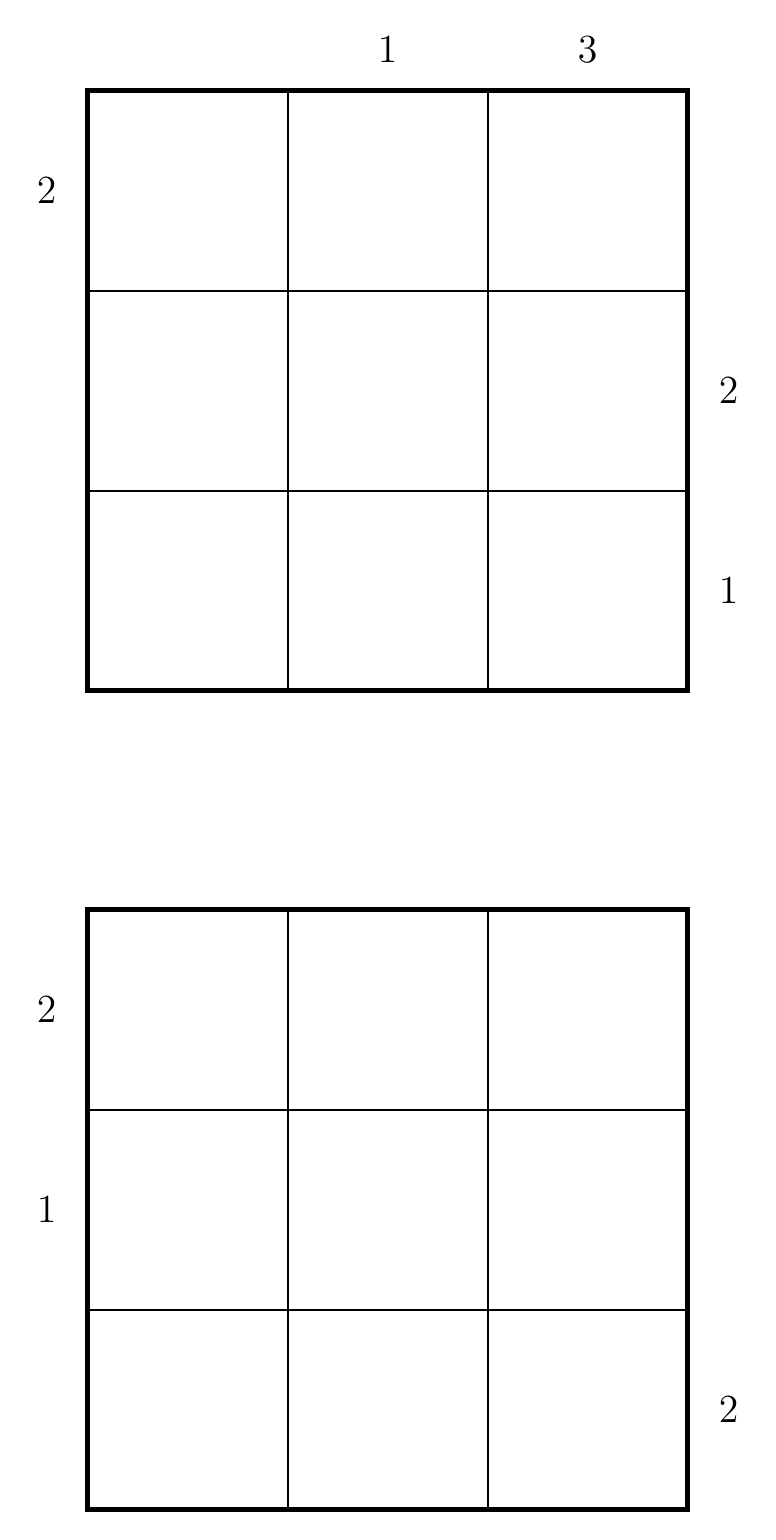
\begin{tikzpicture}
\begin{scope}[shift={(0.000,0.000)}]
\draw[line width=0.7pt] (2.540,0) -- (2.540,7.620);
\draw[line width=0.7pt] (0,2.540) -- (7.620,2.540);
\draw[line width=0.7pt] (5.080,0) -- (5.080,7.620);
\draw[line width=0.7pt] (0,5.080) -- (7.620,5.080);
\draw[line width=1.6pt] (0,0) rectangle (7.620,7.620);
\node at (3.810,8.140) {\Large 1};
\node at (6.350,8.140) {\Large 3};
\node at (-0.520,6.350) {\Large 2};
\node at (8.140,3.810) {\Large 2};
\node at (8.140,1.270) {\Large 1};
\end{scope}
\begin{scope}[shift={(0.000,-10.400)}]
\draw[line width=0.7pt] (2.540,0) -- (2.540,7.620);
\draw[line width=0.7pt] (0,2.540) -- (7.620,2.540);
\draw[line width=0.7pt] (5.080,0) -- (5.080,7.620);
\draw[line width=0.7pt] (0,5.080) -- (7.620,5.080);
\draw[line width=1.6pt] (0,0) rectangle (7.620,7.620);
\node at (-0.520,6.350) {\Large 2};
\node at (-0.520,3.810) {\Large 1};
\node at (8.140,1.270) {\Large 2};
\end{scope}
\end{tikzpicture}
\end{center}
\end{minipage}
\par\vspace{0.75cm}
\newpage
\vspace*{0.3cm}
\begin{center}
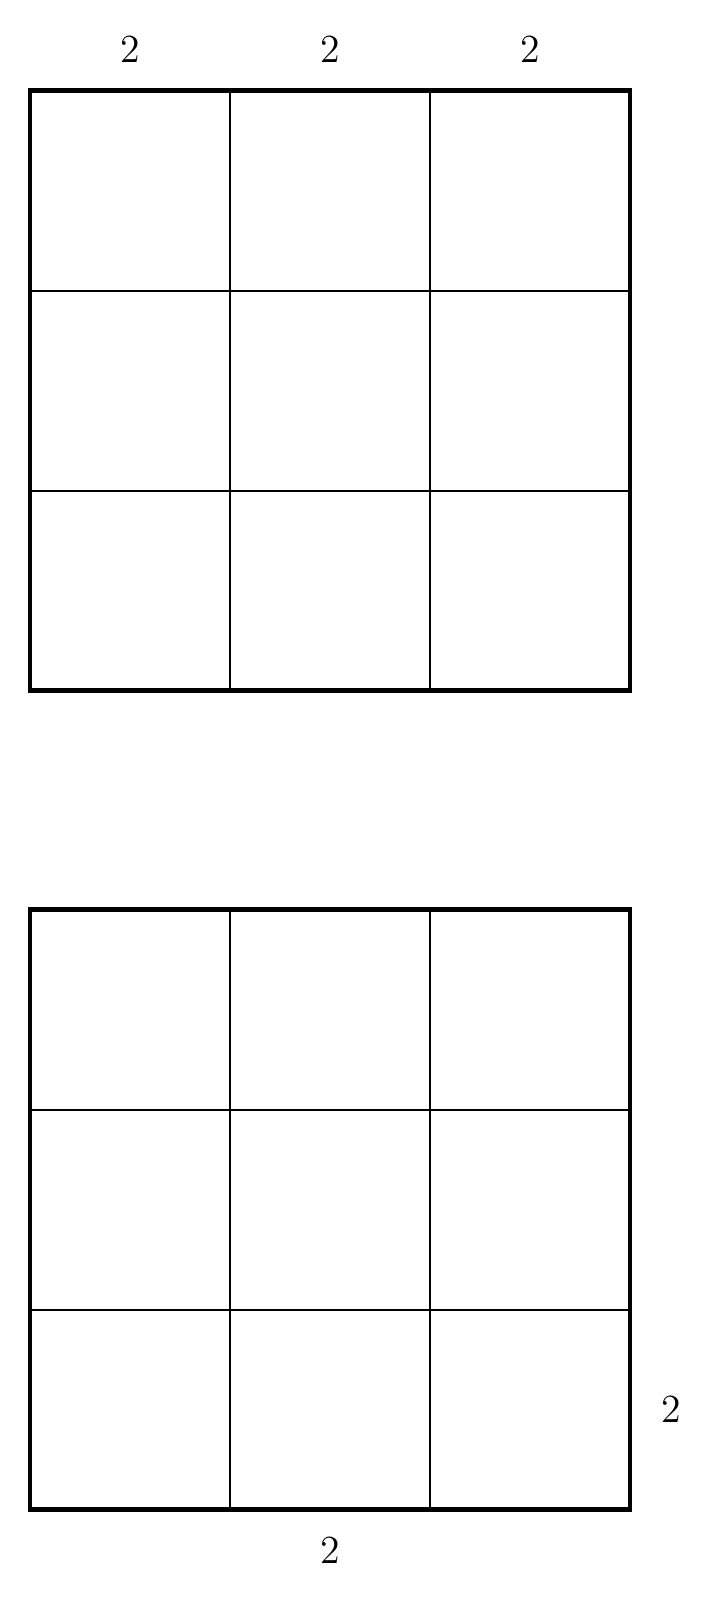
\begin{tikzpicture}
\begin{scope}[shift={(0.000,0.000)}]
\draw[line width=0.7pt] (2.540,0) -- (2.540,7.620);
\draw[line width=0.7pt] (0,2.540) -- (7.620,2.540);
\draw[line width=0.7pt] (5.080,0) -- (5.080,7.620);
\draw[line width=0.7pt] (0,5.080) -- (7.620,5.080);
\draw[line width=1.6pt] (0,0) rectangle (7.620,7.620);
\node at (1.270,8.140) {\Large 2};
\node at (3.810,8.140) {\Large 2};
\node at (6.350,8.140) {\Large 2};
\end{scope}
\begin{scope}[shift={(0.000,-10.400)}]
\draw[line width=0.7pt] (2.540,0) -- (2.540,7.620);
\draw[line width=0.7pt] (0,2.540) -- (7.620,2.540);
\draw[line width=0.7pt] (5.080,0) -- (5.080,7.620);
\draw[line width=0.7pt] (0,5.080) -- (7.620,5.080);
\draw[line width=1.6pt] (0,0) rectangle (7.620,7.620);
\node at (3.810,-0.520) {\Large 2};
\node at (8.140,1.270) {\Large 2};
\end{scope}
\end{tikzpicture}
\end{center}
\newpage
\begin{minipage}{\linewidth}\RaggedRight
\prob{4}More than one city fits the numbers around this grid. Find every city that fits. Then write one more number around the grid so that only one of your cities fits.
\vspace*{0.2cm}
\begin{center}
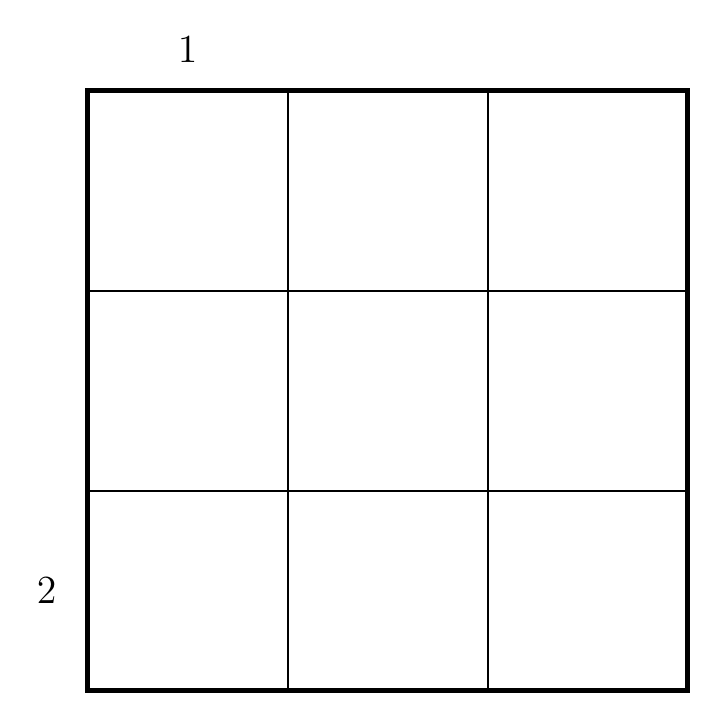
\begin{tikzpicture}
\draw[line width=0.7pt] (2.540,0) -- (2.540,7.620);
\draw[line width=0.7pt] (0,2.540) -- (7.620,2.540);
\draw[line width=0.7pt] (5.080,0) -- (5.080,7.620);
\draw[line width=0.7pt] (0,5.080) -- (7.620,5.080);
\draw[line width=1.6pt] (0,0) rectangle (7.620,7.620);
\node at (1.270,8.140) {\Large 1};
\node at (-0.520,1.270) {\Large 2};
\end{tikzpicture}
\end{center}
\vspace*{0.4cm}
\begin{center}
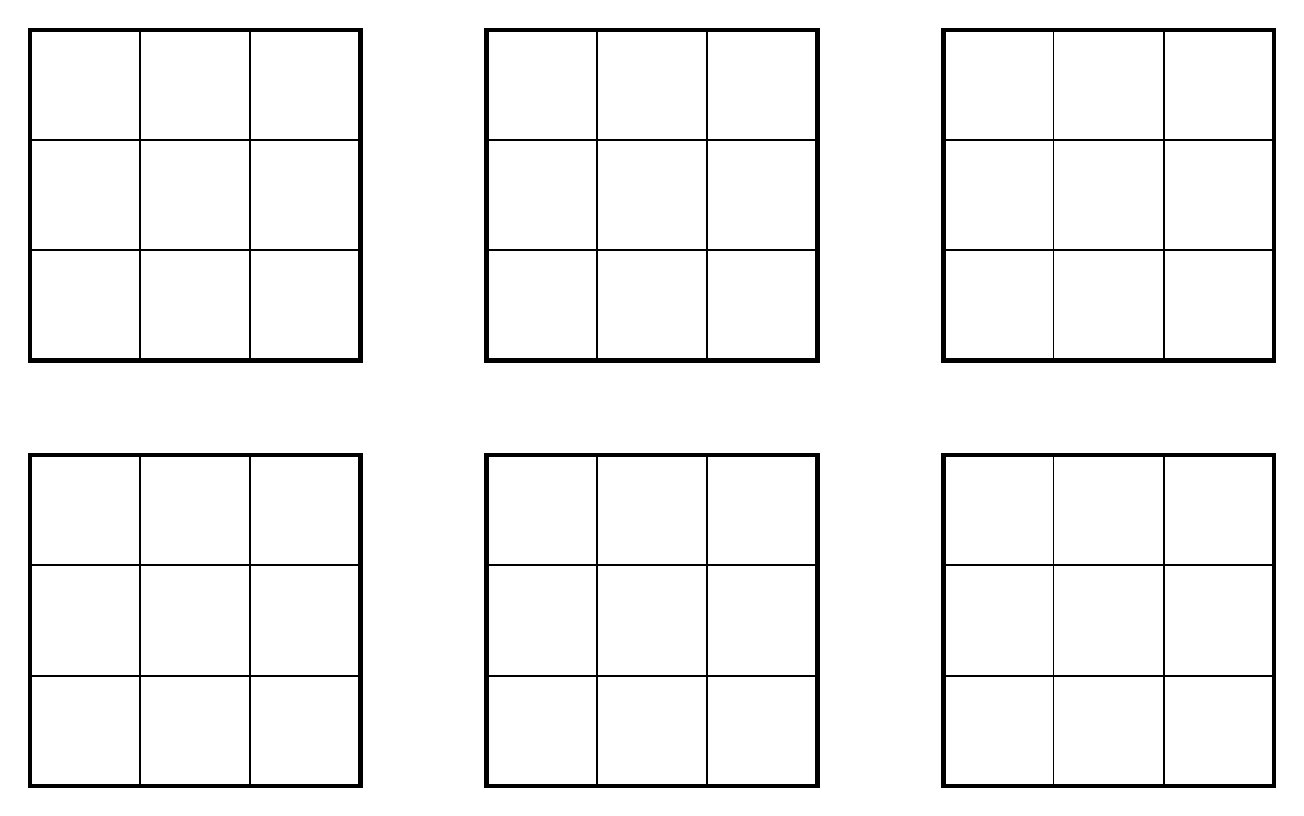
\begin{tikzpicture}
\begin{scope}[shift={(0.000,0.000)}]
\draw[line width=0.7pt] (1.400,0) -- (1.400,4.200);
\draw[line width=0.7pt] (0,1.400) -- (4.200,1.400);
\draw[line width=0.7pt] (2.800,0) -- (2.800,4.200);
\draw[line width=0.7pt] (0,2.800) -- (4.200,2.800);
\draw[line width=1.6pt] (0,0) rectangle (4.200,4.200);
\end{scope}
\begin{scope}[shift={(5.800,0.000)}]
\draw[line width=0.7pt] (1.400,0) -- (1.400,4.200);
\draw[line width=0.7pt] (0,1.400) -- (4.200,1.400);
\draw[line width=0.7pt] (2.800,0) -- (2.800,4.200);
\draw[line width=0.7pt] (0,2.800) -- (4.200,2.800);
\draw[line width=1.6pt] (0,0) rectangle (4.200,4.200);
\end{scope}
\begin{scope}[shift={(11.600,0.000)}]
\draw[line width=0.7pt] (1.400,0) -- (1.400,4.200);
\draw[line width=0.7pt] (0,1.400) -- (4.200,1.400);
\draw[line width=0.7pt] (2.800,0) -- (2.800,4.200);
\draw[line width=0.7pt] (0,2.800) -- (4.200,2.800);
\draw[line width=1.6pt] (0,0) rectangle (4.200,4.200);
\end{scope}
\begin{scope}[shift={(0.000,-5.400)}]
\draw[line width=0.7pt] (1.400,0) -- (1.400,4.200);
\draw[line width=0.7pt] (0,1.400) -- (4.200,1.400);
\draw[line width=0.7pt] (2.800,0) -- (2.800,4.200);
\draw[line width=0.7pt] (0,2.800) -- (4.200,2.800);
\draw[line width=1.6pt] (0,0) rectangle (4.200,4.200);
\end{scope}
\begin{scope}[shift={(5.800,-5.400)}]
\draw[line width=0.7pt] (1.400,0) -- (1.400,4.200);
\draw[line width=0.7pt] (0,1.400) -- (4.200,1.400);
\draw[line width=0.7pt] (2.800,0) -- (2.800,4.200);
\draw[line width=0.7pt] (0,2.800) -- (4.200,2.800);
\draw[line width=1.6pt] (0,0) rectangle (4.200,4.200);
\end{scope}
\begin{scope}[shift={(11.600,-5.400)}]
\draw[line width=0.7pt] (1.400,0) -- (1.400,4.200);
\draw[line width=0.7pt] (0,1.400) -- (4.200,1.400);
\draw[line width=0.7pt] (2.800,0) -- (2.800,4.200);
\draw[line width=0.7pt] (0,2.800) -- (4.200,2.800);
\draw[line width=1.6pt] (0,0) rectangle (4.200,4.200);
\end{scope}
\end{tikzpicture}
\end{center}
\end{minipage}
\par\vspace{0.75cm}
\newpage
\begin{minipage}{\linewidth}\RaggedRight
\prob{5}Build a city behind a folder, out of your partner's sight. Write some of its numbers around an empty grid so that your city is the only one that fits. Your partner solves the puzzle and tries to find a second city that fits the same numbers. How few numbers can a puzzle have and still fit only one city? Explain why fewer cannot work.
\vspace*{0.1cm}
\begin{center}
\begin{tikzpicture}
\begin{scope}[shift={(0.000,0.000)}]
\draw[line width=0.7pt] (2.540,0) -- (2.540,7.620);
\draw[line width=0.7pt] (0,2.540) -- (7.620,2.540);
\draw[line width=0.7pt] (5.080,0) -- (5.080,7.620);
\draw[line width=0.7pt] (0,5.080) -- (7.620,5.080);
\draw[line width=1.6pt] (0,0) rectangle (7.620,7.620);
\draw[black!45, line width=0.6pt] (0.895,7.900) rectangle (1.645,8.650);
\draw[black!45, line width=0.6pt] (3.435,7.900) rectangle (4.185,8.650);
\draw[black!45, line width=0.6pt] (5.975,7.900) rectangle (6.725,8.650);
\draw[black!45, line width=0.6pt] (0.895,-1.030) rectangle (1.645,-0.280);
\draw[black!45, line width=0.6pt] (3.435,-1.030) rectangle (4.185,-0.280);
\draw[black!45, line width=0.6pt] (5.975,-1.030) rectangle (6.725,-0.280);
\draw[black!45, line width=0.6pt] (-1.030,5.975) rectangle (-0.280,6.725);
\draw[black!45, line width=0.6pt] (-1.030,3.435) rectangle (-0.280,4.185);
\draw[black!45, line width=0.6pt] (-1.030,0.895) rectangle (-0.280,1.645);
\draw[black!45, line width=0.6pt] (7.900,5.975) rectangle (8.650,6.725);
\draw[black!45, line width=0.6pt] (7.900,3.435) rectangle (8.650,4.185);
\draw[black!45, line width=0.6pt] (7.900,0.895) rectangle (8.650,1.645);
\end{scope}
\begin{scope}[shift={(8.300,-10.220)}]
\draw[line width=0.7pt] (2.540,0) -- (2.540,7.620);
\draw[line width=0.7pt] (0,2.540) -- (7.620,2.540);
\draw[line width=0.7pt] (5.080,0) -- (5.080,7.620);
\draw[line width=0.7pt] (0,5.080) -- (7.620,5.080);
\draw[line width=1.6pt] (0,0) rectangle (7.620,7.620);
\draw[black!45, line width=0.6pt] (0.895,7.900) rectangle (1.645,8.650);
\draw[black!45, line width=0.6pt] (3.435,7.900) rectangle (4.185,8.650);
\draw[black!45, line width=0.6pt] (5.975,7.900) rectangle (6.725,8.650);
\draw[black!45, line width=0.6pt] (0.895,-1.030) rectangle (1.645,-0.280);
\draw[black!45, line width=0.6pt] (3.435,-1.030) rectangle (4.185,-0.280);
\draw[black!45, line width=0.6pt] (5.975,-1.030) rectangle (6.725,-0.280);
\draw[black!45, line width=0.6pt] (-1.030,5.975) rectangle (-0.280,6.725);
\draw[black!45, line width=0.6pt] (-1.030,3.435) rectangle (-0.280,4.185);
\draw[black!45, line width=0.6pt] (-1.030,0.895) rectangle (-0.280,1.645);
\draw[black!45, line width=0.6pt] (7.900,5.975) rectangle (8.650,6.725);
\draw[black!45, line width=0.6pt] (7.900,3.435) rectangle (8.650,4.185);
\draw[black!45, line width=0.6pt] (7.900,0.895) rectangle (8.650,1.645);
\end{scope}
\end{tikzpicture}
\end{center}
\end{minipage}
\par\vspace{0.75cm}
\newpage
\vspace*{0.6cm}
\begin{center}
\begin{tikzpicture}
\begin{scope}[shift={(0.000,0.000)}]
\draw[line width=0.7pt] (2.540,0) -- (2.540,7.620);
\draw[line width=0.7pt] (0,2.540) -- (7.620,2.540);
\draw[line width=0.7pt] (5.080,0) -- (5.080,7.620);
\draw[line width=0.7pt] (0,5.080) -- (7.620,5.080);
\draw[line width=1.6pt] (0,0) rectangle (7.620,7.620);
\draw[black!45, line width=0.6pt] (0.895,7.900) rectangle (1.645,8.650);
\draw[black!45, line width=0.6pt] (3.435,7.900) rectangle (4.185,8.650);
\draw[black!45, line width=0.6pt] (5.975,7.900) rectangle (6.725,8.650);
\draw[black!45, line width=0.6pt] (0.895,-1.030) rectangle (1.645,-0.280);
\draw[black!45, line width=0.6pt] (3.435,-1.030) rectangle (4.185,-0.280);
\draw[black!45, line width=0.6pt] (5.975,-1.030) rectangle (6.725,-0.280);
\draw[black!45, line width=0.6pt] (-1.030,5.975) rectangle (-0.280,6.725);
\draw[black!45, line width=0.6pt] (-1.030,3.435) rectangle (-0.280,4.185);
\draw[black!45, line width=0.6pt] (-1.030,0.895) rectangle (-0.280,1.645);
\draw[black!45, line width=0.6pt] (7.900,5.975) rectangle (8.650,6.725);
\draw[black!45, line width=0.6pt] (7.900,3.435) rectangle (8.650,4.185);
\draw[black!45, line width=0.6pt] (7.900,0.895) rectangle (8.650,1.645);
\end{scope}
\begin{scope}[shift={(8.300,-11.000)}]
\draw[line width=0.7pt] (2.540,0) -- (2.540,7.620);
\draw[line width=0.7pt] (0,2.540) -- (7.620,2.540);
\draw[line width=0.7pt] (5.080,0) -- (5.080,7.620);
\draw[line width=0.7pt] (0,5.080) -- (7.620,5.080);
\draw[line width=1.6pt] (0,0) rectangle (7.620,7.620);
\draw[black!45, line width=0.6pt] (0.895,7.900) rectangle (1.645,8.650);
\draw[black!45, line width=0.6pt] (3.435,7.900) rectangle (4.185,8.650);
\draw[black!45, line width=0.6pt] (5.975,7.900) rectangle (6.725,8.650);
\draw[black!45, line width=0.6pt] (0.895,-1.030) rectangle (1.645,-0.280);
\draw[black!45, line width=0.6pt] (3.435,-1.030) rectangle (4.185,-0.280);
\draw[black!45, line width=0.6pt] (5.975,-1.030) rectangle (6.725,-0.280);
\draw[black!45, line width=0.6pt] (-1.030,5.975) rectangle (-0.280,6.725);
\draw[black!45, line width=0.6pt] (-1.030,3.435) rectangle (-0.280,4.185);
\draw[black!45, line width=0.6pt] (-1.030,0.895) rectangle (-0.280,1.645);
\draw[black!45, line width=0.6pt] (7.900,5.975) rectangle (8.650,6.725);
\draw[black!45, line width=0.6pt] (7.900,3.435) rectangle (8.650,4.185);
\draw[black!45, line width=0.6pt] (7.900,0.895) rectangle (8.650,1.645);
\end{scope}
\end{tikzpicture}
\end{center}
\newpage
\begin{minipage}{\linewidth}\RaggedRight
\prob{6}How many different 3-by-3 cities are there? Cities that are turned or flipped count as different. Write each city you find in a grid. Explain how you know you have found them all.
\vspace*{0.3cm}
\begin{center}
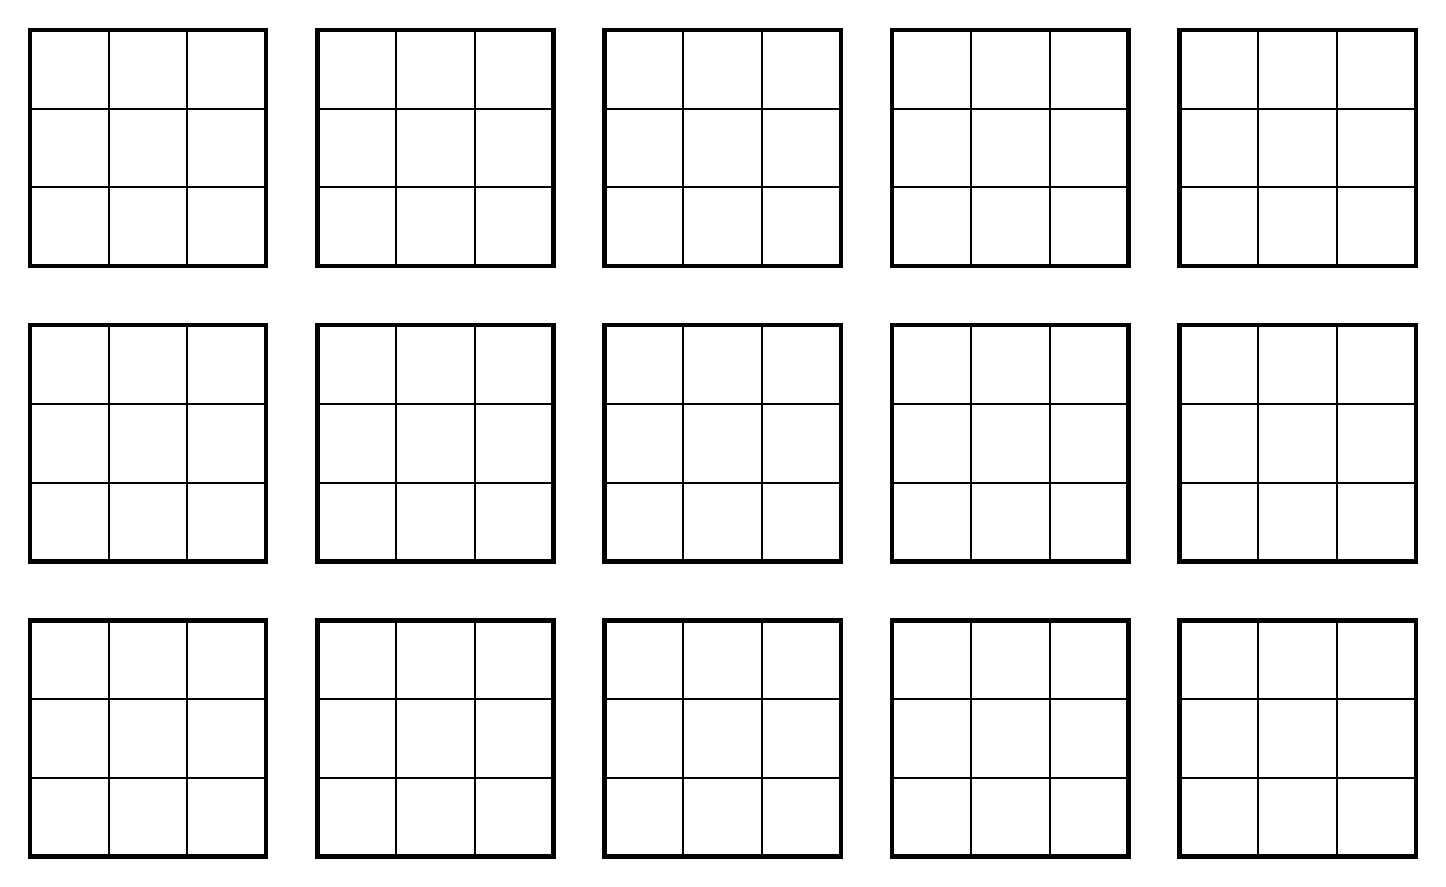
\begin{tikzpicture}
\begin{scope}[shift={(0.000,0.000)}]
\draw[line width=0.7pt] (1.000,0) -- (1.000,3.000);
\draw[line width=0.7pt] (0,1.000) -- (3.000,1.000);
\draw[line width=0.7pt] (2.000,0) -- (2.000,3.000);
\draw[line width=0.7pt] (0,2.000) -- (3.000,2.000);
\draw[line width=1.6pt] (0,0) rectangle (3.000,3.000);
\end{scope}
\begin{scope}[shift={(3.650,0.000)}]
\draw[line width=0.7pt] (1.000,0) -- (1.000,3.000);
\draw[line width=0.7pt] (0,1.000) -- (3.000,1.000);
\draw[line width=0.7pt] (2.000,0) -- (2.000,3.000);
\draw[line width=0.7pt] (0,2.000) -- (3.000,2.000);
\draw[line width=1.6pt] (0,0) rectangle (3.000,3.000);
\end{scope}
\begin{scope}[shift={(7.300,0.000)}]
\draw[line width=0.7pt] (1.000,0) -- (1.000,3.000);
\draw[line width=0.7pt] (0,1.000) -- (3.000,1.000);
\draw[line width=0.7pt] (2.000,0) -- (2.000,3.000);
\draw[line width=0.7pt] (0,2.000) -- (3.000,2.000);
\draw[line width=1.6pt] (0,0) rectangle (3.000,3.000);
\end{scope}
\begin{scope}[shift={(10.950,0.000)}]
\draw[line width=0.7pt] (1.000,0) -- (1.000,3.000);
\draw[line width=0.7pt] (0,1.000) -- (3.000,1.000);
\draw[line width=0.7pt] (2.000,0) -- (2.000,3.000);
\draw[line width=0.7pt] (0,2.000) -- (3.000,2.000);
\draw[line width=1.6pt] (0,0) rectangle (3.000,3.000);
\end{scope}
\begin{scope}[shift={(14.600,0.000)}]
\draw[line width=0.7pt] (1.000,0) -- (1.000,3.000);
\draw[line width=0.7pt] (0,1.000) -- (3.000,1.000);
\draw[line width=0.7pt] (2.000,0) -- (2.000,3.000);
\draw[line width=0.7pt] (0,2.000) -- (3.000,2.000);
\draw[line width=1.6pt] (0,0) rectangle (3.000,3.000);
\end{scope}
\begin{scope}[shift={(0.000,-3.750)}]
\draw[line width=0.7pt] (1.000,0) -- (1.000,3.000);
\draw[line width=0.7pt] (0,1.000) -- (3.000,1.000);
\draw[line width=0.7pt] (2.000,0) -- (2.000,3.000);
\draw[line width=0.7pt] (0,2.000) -- (3.000,2.000);
\draw[line width=1.6pt] (0,0) rectangle (3.000,3.000);
\end{scope}
\begin{scope}[shift={(3.650,-3.750)}]
\draw[line width=0.7pt] (1.000,0) -- (1.000,3.000);
\draw[line width=0.7pt] (0,1.000) -- (3.000,1.000);
\draw[line width=0.7pt] (2.000,0) -- (2.000,3.000);
\draw[line width=0.7pt] (0,2.000) -- (3.000,2.000);
\draw[line width=1.6pt] (0,0) rectangle (3.000,3.000);
\end{scope}
\begin{scope}[shift={(7.300,-3.750)}]
\draw[line width=0.7pt] (1.000,0) -- (1.000,3.000);
\draw[line width=0.7pt] (0,1.000) -- (3.000,1.000);
\draw[line width=0.7pt] (2.000,0) -- (2.000,3.000);
\draw[line width=0.7pt] (0,2.000) -- (3.000,2.000);
\draw[line width=1.6pt] (0,0) rectangle (3.000,3.000);
\end{scope}
\begin{scope}[shift={(10.950,-3.750)}]
\draw[line width=0.7pt] (1.000,0) -- (1.000,3.000);
\draw[line width=0.7pt] (0,1.000) -- (3.000,1.000);
\draw[line width=0.7pt] (2.000,0) -- (2.000,3.000);
\draw[line width=0.7pt] (0,2.000) -- (3.000,2.000);
\draw[line width=1.6pt] (0,0) rectangle (3.000,3.000);
\end{scope}
\begin{scope}[shift={(14.600,-3.750)}]
\draw[line width=0.7pt] (1.000,0) -- (1.000,3.000);
\draw[line width=0.7pt] (0,1.000) -- (3.000,1.000);
\draw[line width=0.7pt] (2.000,0) -- (2.000,3.000);
\draw[line width=0.7pt] (0,2.000) -- (3.000,2.000);
\draw[line width=1.6pt] (0,0) rectangle (3.000,3.000);
\end{scope}
\begin{scope}[shift={(0.000,-7.500)}]
\draw[line width=0.7pt] (1.000,0) -- (1.000,3.000);
\draw[line width=0.7pt] (0,1.000) -- (3.000,1.000);
\draw[line width=0.7pt] (2.000,0) -- (2.000,3.000);
\draw[line width=0.7pt] (0,2.000) -- (3.000,2.000);
\draw[line width=1.6pt] (0,0) rectangle (3.000,3.000);
\end{scope}
\begin{scope}[shift={(3.650,-7.500)}]
\draw[line width=0.7pt] (1.000,0) -- (1.000,3.000);
\draw[line width=0.7pt] (0,1.000) -- (3.000,1.000);
\draw[line width=0.7pt] (2.000,0) -- (2.000,3.000);
\draw[line width=0.7pt] (0,2.000) -- (3.000,2.000);
\draw[line width=1.6pt] (0,0) rectangle (3.000,3.000);
\end{scope}
\begin{scope}[shift={(7.300,-7.500)}]
\draw[line width=0.7pt] (1.000,0) -- (1.000,3.000);
\draw[line width=0.7pt] (0,1.000) -- (3.000,1.000);
\draw[line width=0.7pt] (2.000,0) -- (2.000,3.000);
\draw[line width=0.7pt] (0,2.000) -- (3.000,2.000);
\draw[line width=1.6pt] (0,0) rectangle (3.000,3.000);
\end{scope}
\begin{scope}[shift={(10.950,-7.500)}]
\draw[line width=0.7pt] (1.000,0) -- (1.000,3.000);
\draw[line width=0.7pt] (0,1.000) -- (3.000,1.000);
\draw[line width=0.7pt] (2.000,0) -- (2.000,3.000);
\draw[line width=0.7pt] (0,2.000) -- (3.000,2.000);
\draw[line width=1.6pt] (0,0) rectangle (3.000,3.000);
\end{scope}
\begin{scope}[shift={(14.600,-7.500)}]
\draw[line width=0.7pt] (1.000,0) -- (1.000,3.000);
\draw[line width=0.7pt] (0,1.000) -- (3.000,1.000);
\draw[line width=0.7pt] (2.000,0) -- (2.000,3.000);
\draw[line width=0.7pt] (0,2.000) -- (3.000,2.000);
\draw[line width=1.6pt] (0,0) rectangle (3.000,3.000);
\end{scope}
\end{tikzpicture}
\end{center}
\end{minipage}
\par\vspace{0.75cm}
\newpage
\begin{minipage}{\linewidth}\RaggedRight
\prob{7}Add up the twelve numbers around a 3-by-3 city. Which totals can a city have? Explain why.
\vspace*{0.3cm}
\begin{center}
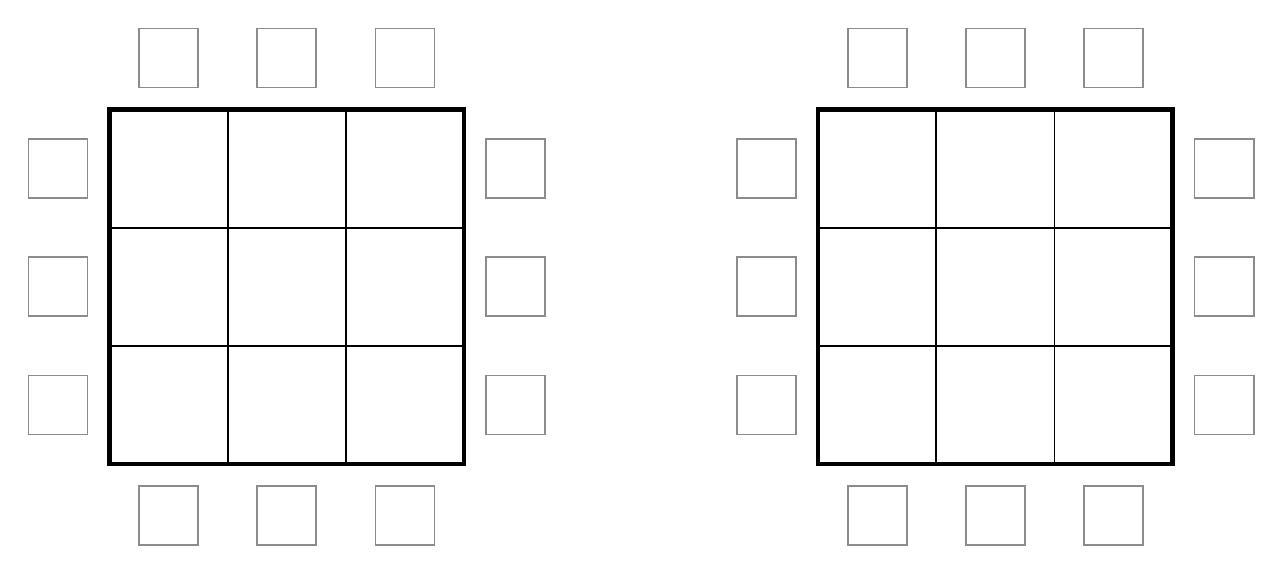
\begin{tikzpicture}
\begin{scope}[shift={(0.000,0.000)}]
\draw[line width=0.7pt] (1.500,0) -- (1.500,4.500);
\draw[line width=0.7pt] (0,1.500) -- (4.500,1.500);
\draw[line width=0.7pt] (3.000,0) -- (3.000,4.500);
\draw[line width=0.7pt] (0,3.000) -- (4.500,3.000);
\draw[line width=1.6pt] (0,0) rectangle (4.500,4.500);
\draw[black!45, line width=0.6pt] (0.375,4.780) rectangle (1.125,5.530);
\draw[black!45, line width=0.6pt] (1.875,4.780) rectangle (2.625,5.530);
\draw[black!45, line width=0.6pt] (3.375,4.780) rectangle (4.125,5.530);
\draw[black!45, line width=0.6pt] (0.375,-1.030) rectangle (1.125,-0.280);
\draw[black!45, line width=0.6pt] (1.875,-1.030) rectangle (2.625,-0.280);
\draw[black!45, line width=0.6pt] (3.375,-1.030) rectangle (4.125,-0.280);
\draw[black!45, line width=0.6pt] (-1.030,3.375) rectangle (-0.280,4.125);
\draw[black!45, line width=0.6pt] (-1.030,1.875) rectangle (-0.280,2.625);
\draw[black!45, line width=0.6pt] (-1.030,0.375) rectangle (-0.280,1.125);
\draw[black!45, line width=0.6pt] (4.780,3.375) rectangle (5.530,4.125);
\draw[black!45, line width=0.6pt] (4.780,1.875) rectangle (5.530,2.625);
\draw[black!45, line width=0.6pt] (4.780,0.375) rectangle (5.530,1.125);
\end{scope}
\begin{scope}[shift={(9.000,0.000)}]
\draw[line width=0.7pt] (1.500,0) -- (1.500,4.500);
\draw[line width=0.7pt] (0,1.500) -- (4.500,1.500);
\draw[line width=0.7pt] (3.000,0) -- (3.000,4.500);
\draw[line width=0.7pt] (0,3.000) -- (4.500,3.000);
\draw[line width=1.6pt] (0,0) rectangle (4.500,4.500);
\draw[black!45, line width=0.6pt] (0.375,4.780) rectangle (1.125,5.530);
\draw[black!45, line width=0.6pt] (1.875,4.780) rectangle (2.625,5.530);
\draw[black!45, line width=0.6pt] (3.375,4.780) rectangle (4.125,5.530);
\draw[black!45, line width=0.6pt] (0.375,-1.030) rectangle (1.125,-0.280);
\draw[black!45, line width=0.6pt] (1.875,-1.030) rectangle (2.625,-0.280);
\draw[black!45, line width=0.6pt] (3.375,-1.030) rectangle (4.125,-0.280);
\draw[black!45, line width=0.6pt] (-1.030,3.375) rectangle (-0.280,4.125);
\draw[black!45, line width=0.6pt] (-1.030,1.875) rectangle (-0.280,2.625);
\draw[black!45, line width=0.6pt] (-1.030,0.375) rectangle (-0.280,1.125);
\draw[black!45, line width=0.6pt] (4.780,3.375) rectangle (5.530,4.125);
\draw[black!45, line width=0.6pt] (4.780,1.875) rectangle (5.530,2.625);
\draw[black!45, line width=0.6pt] (4.780,0.375) rectangle (5.530,1.125);
\end{scope}
\end{tikzpicture}
\end{center}
\end{minipage}
\par\vspace{0.75cm}
\end{document}
